\subsection{Aliasing Adventures: Unveiling Waveform Wonders on Your Oscilloscope!}

\begin{tcolorbox}[colback=gray!10, colframe=black, title=E4A06] What is the effect of aliasing on a digital oscilloscope when displaying a waveform?

\begin{enumerate}[label=\Alph*.]
    \item \textbf{A} A false, jittery low-frequency version of the waveform is displayed
    \item B The waveform DC offset will be inaccurate
    \item C Calibration of the vertical scale is no longer valid
    \item D Excessive blanking occurs, which prevents display of the waveform
\end{enumerate} \end{tcolorbox}

\subsubsection{Understanding Aliasing}
Aliasing is a phenomenon that occurs when a signal is sampled at a rate that is insufficient to capture its variations accurately. In the context of a digital oscilloscope, this means that the sampling frequency must be at least twice the highest frequency present in the waveform, as per the Nyquist-Shannon sampling theorem. If the sampling frequency is lower than this threshold, the representation of the waveform may not reflect the actual shape of the signal, leading to misinterpretations.

When aliasing occurs, the displayed waveform may appear as a false low-frequency signal—this confusion manifests as a pulse or jitter in the shape of the waveform that is not present in the original signal. This is particularly significant in the measurement and analysis of high-frequency signals, where accurate representation is critical.

\subsubsection{Effects of Aliasing}
Among the choices given, option A accurately describes the consequence of aliasing on the waveform display of a digital oscilloscope. Unlike the other choices that pertain to inaccuracies or calibration issues, aliasing specifically affects how the waveform appears due to inadequate sampling rates.

To illustrate, let's consider a scenario where a waveform of frequency \( f \) is sampled at a sampling frequency \( f_s \):

1. When \( f_s < 2f \), aliasing occurs.
2. If \( f = 1 \, \text{kHz} \) and we sample at \( f_s = 1.5 \, \text{kHz} \), the condition \( f_s < 2f \) holds. Therefore, the oscilloscope may show a false representation of the waveform.

The mathematical representation can be further exemplified as follows:

- If the original signal is a sinusoid \( x(t) = A \sin(2\pi f t) \),
- The sampled signal can be represented as \( x[n] = x(nT) = A \sin(2\pi f nT) \) where \( T = \frac{1}{f_s} \).

If \( T \) is too large (low \( f_s \)), the sine function may appear different when reconstructed, leading to a misleading output that looks like low-frequency oscillations despite being a high-frequency input.

\subsubsection{Conclusion}
Understanding the effect of aliasing is crucial for effectively using digital oscilloscopes, particularly in applications involving high-frequency signals. Without adequate sampling, the displayed waveform can lead to significant errors in interpretation and measurement, which subsequently affects the overall signal analysis, diagnostics, and troubleshooting in electronic systems.

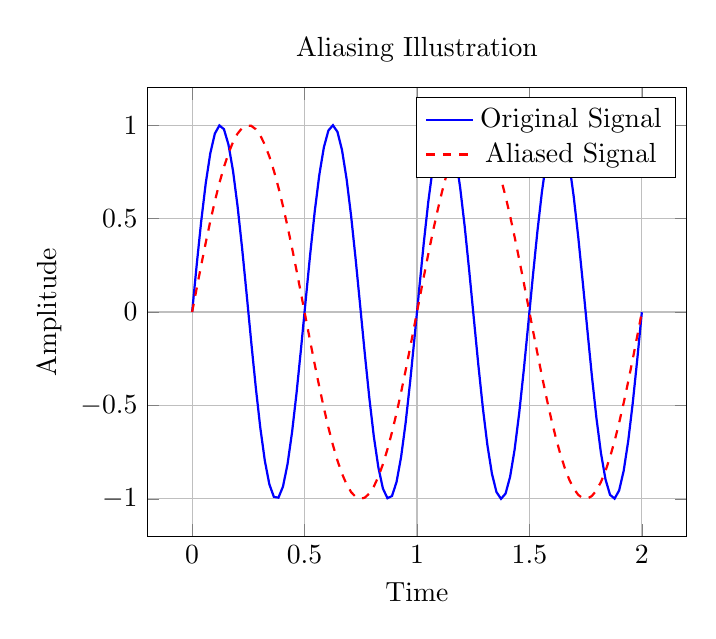
\begin{tikzpicture}
    \begin{axis}[
        title={Aliasing Illustration},
        xlabel={Time},
        ylabel={Amplitude},
        grid=major,
        domain=0:2,
        samples=100
    ]
    \addplot[blue, thick] {sin(deg(2*pi*2*x))}; % Original signal
    \addplot[red, thick, dashed] {sin(deg(2*pi*1*x))}; % Sampled signal with aliasing
    \legend{Original Signal, Aliased Signal}
    \end{axis}
\end{tikzpicture}
